\documentclass[11pt,spanish,a4paper]{article}
\usepackage[utf8]{inputenc}
\usepackage[spanish,es-nodecimaldot]{babel}
\usepackage{times}
\usepackage{graphicx}
\usepackage{amsmath,amssymb}
\usepackage{multicol}
\oddsidemargin=0.5cm
\textwidth=15cm
\textheight=50\baselineskip
\topmargin=-1.5cm
\parskip 1em
%\parindent 0pt

\begin{document}
%\renewcommand{\labelenumi}{\em \alph{enumi})}
%\renewcommand{\labelenumii}{\em \arabic{enumii})}
\newcommand\al{\alpha}
\newcommand\noi{\noindent}
\newcommand\re{\mbox{Re}}
\newcommand\im{\mbox{Im}}
%\newcommand\arg{\mbox{arg}}
\newcommand\Arg{\mbox{Arg}}


\title{Proyecciones en $\mathbb{R}^2$}
\author{Matías Valle}
\maketitle


\begin{abstract}
En este trabajo nos orientaremos hacia la explicion de lo que son las proyecciones en $\mathbb{R}^2$, tratando de explayar lo mas claro posible el concepto, para que el que lea este documento pueda saber y conocer sobre el tema.Se trataran todos los temas que se crean necesarios para su comprension, como tambien las caracteristicas del tema que sea considerada importante para el autor.
\end{abstract}

\begin{center}
\section{Introducción}
Las proyecciones son un importante componente de las matematicas(como casi todo tema que la integra), sobre todo para estudiar espacios vectoriales, planos, longitudes, magnitudes, etcetera.Trataremos de centrarnos en los temas mas globales sobre el tema, para asi poder dar un conocimiento general de este concepto y que quede lo mas claro posible, tratando de no explayarnos demasiado en conceptos muy metodicos, e intentar ir a lo general.
\end{center}

\section{Proyecciones}
Una proyección es un mapeo de un conjunto(o de algnua estructura matematica) el cual es idempotente, es decir, que la proyeccion es igual a la composicion con ella misma.Tenemos diferentes definiciones de preyeccion depende sobre que parte del tema estemos tranajando:
\itemize


\item Definimos un espacio vectorial V con producto interno, y sean u y v $\epsilon$ V, podemos definir la proyeccion de u sobre v como:
\[proy_v u =\frac{(u/v)}{v/v}v \]

\item Sea V un espacio vectorial, talque $V = v_1 \oplus v_2$, con $v_1$ y $v_2$ subespacios de V, definimos la transformacion lineal $P:V \rightarrow V$ :
\[P(v_1 + v_2) = v_1 (v_1 \epsilon V_1, v_2 \epsilon V_2)\]
En este caso se dice que $P$ es la proyeccion a $v_1$ paralela a $v_2$.Con esto podemos demostrar que si $P: V \rightarrow V$ es proyección, enotnces $P$ se dice que es Idempotente(Se define que un operador lineal es idempotente si $P^2 = P$).

\underline{Demostracion:} \linebreak
Sea $\alpha \epsilon V$ , $\alpha = \alpha_1 + \alpha_2$ ,con $\alpha_1 \epsilon V_1$ , $\alpha_2 \epsilon V_2$,sabiendo que $P(\alpha)= \alpha_1$ : \linebreak

\begin{eqnarray*}
(P \circ P) (\alpha) & = & P(P(\alpha))\\
& = & P(\alpha_1)\\
& = & \alpha_1\\
\end{eqnarray*}

Por lo tanto obtenemos que $P(\alpha) = (P \circ P)(\alpha)$ , y por lo tanto $P$ es idemotente.
\linebreak
\linebreak

En otros terminos mas "vagos", se puede expresar la proyeccion de un vector sobre otro trazando una linea recta desde el vector "superior" hacia el vector "inferior", formando asi un angulo de $90^\circ$ , diciendose que la sombra del vector "superior" esta reflejada sobre la del vector "inferior", llamandose a esto la proyeccion de un vector sobre otro.
Para reflejar mejor estas definiciones y verlo de manera mas grafica, propondremos un par de ejemplos que anexaremos mas abajo, para que la comprension del tema no sea solo escrita, si no, que con con imagenes(o graficos), se entienda mejor de los que estamos hablando.

\subsection{Graficos de Proyecciones}
En esta sección mostraremos un par de graficos de proyecciones para que se pueda ver de manera mas clara lo que se representa graficamente cuando hablamos de una proyecciones.Para ello representaremos mediante graficos hechos en Phython proyecciones para poder verlos de manera mas clara.
\begin{enumerate}

\item En el primer grafico veremos los vectores $u=(5,2)$ y $v= (2,3)$, con origen en el punto $A =(0,0)$ del eje de coordenadas y mostraremos cual es la proyeccion del vector $v$ sobre el vector $u$.

\begin{figure}[h]
\begin{center}
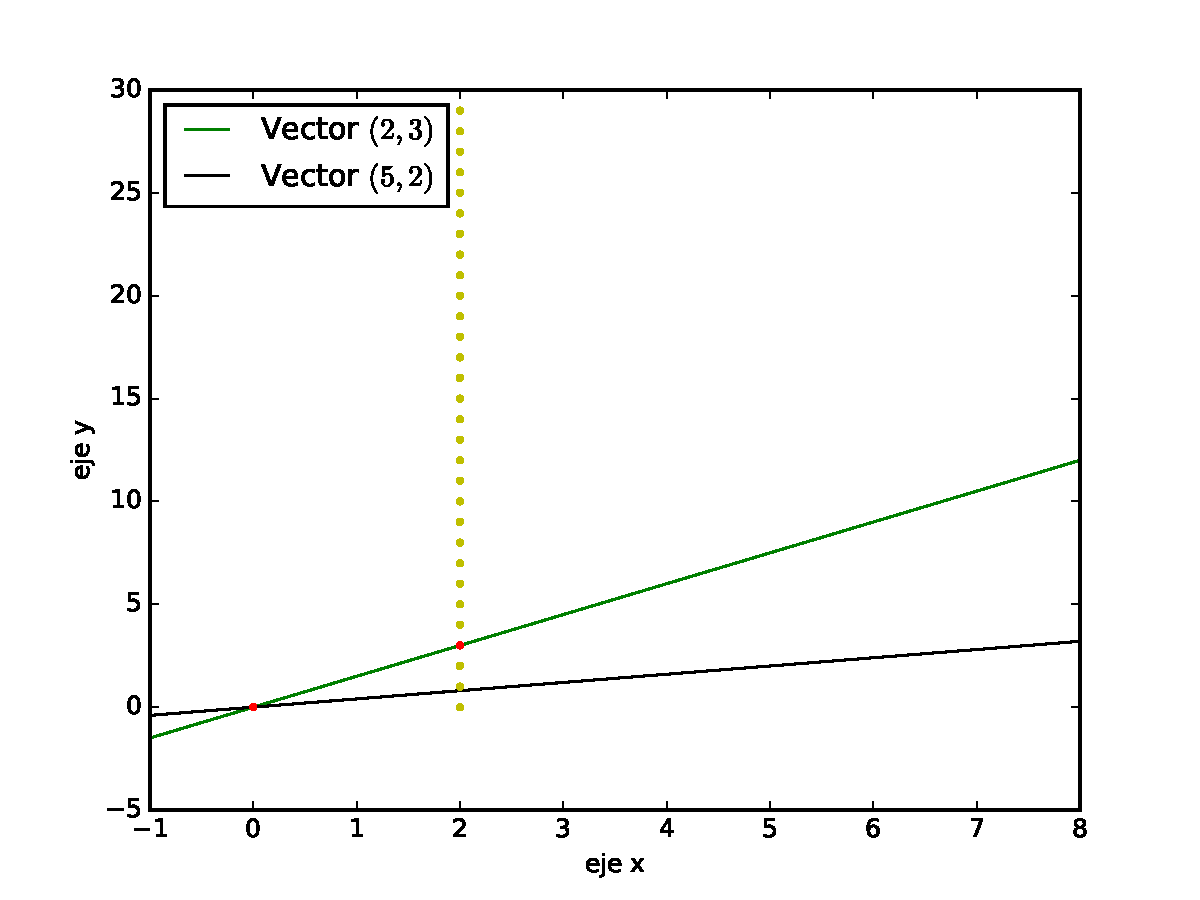
\includegraphics[width=7cm]{graf1.pdf}
\caption{Proyeccion delvector $v$ sobre el vector $u$ }\label{plot1}
\end{center}
\end{figure}

Como vemos en la imagen la proyeccion del vector $v$ sobre $u$, va desde el punto $A=(0,0)$ hasta la linea punteada amarilla, que pasa verticalmente por el punto $(2,3)$ del vector v, cortando el vector $u$. 

\item En este segundo caso veremos un ejemplo parecido pero con distintos vectores, para asi poder apreciar desde otro punto de vista y sea mas amplia la interpretacion de los ejemplos.En este caso tendremos los vectores $v=(4,1)$ y $W=(1,6)$.Como ya hemos dicho anteriormente, tambien tendran su punto de inicio en el punto de origen $A=(0,0)$, y mostraremos la proyeccion del vector $w$ sobre el vector $V$.

\begin{figure}[h]
\begin{center}
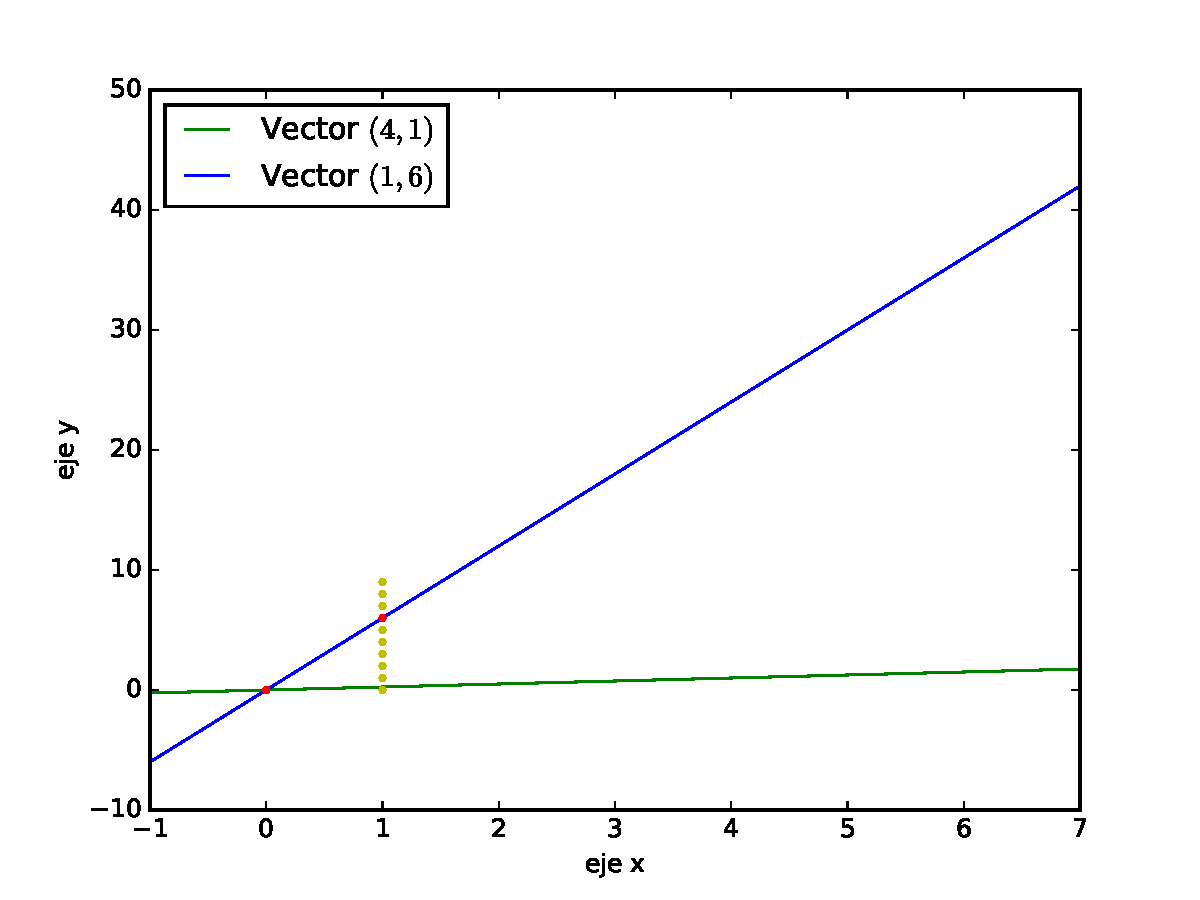
\includegraphics[width=9cm]{graf2.pdf}
\caption{Proyeccion delvector $w$ sobre el vector $v$ }\label{plot1}
\end{center}
\end{figure}
\end{enumerate}

En el caso del ejemplo 2, es similar al ejemplo 1, pero con distintos vectores. Vemos que la proyeccion del vector $w$ sobre $v$, va desde el punto $A=(0,0)$, hasta la linea puntuada que pasa verticalmente por el punto $(1,6)$ del vector $w$.



\subsection{Aclaraciones sobre graficos}
A pesar que en los ejemplos vimos que los vectores comenzaban desde el punto de origen del plano, debemos tener en cuenta que esto no es estrictamente necesario, ya que se puede encontrar la proyeccion de un vector sobre otro, sea donde sea que esten en el plano, tomando en cuenta que estos vectores deben cumplir la condicion de tener un punto en comun para tomar la proyección. 

\break
\section{Conclusiones}
En este trabajo hemos intentado dejar el claro que es y de que se trata cuando hablamos de proyecciones en matemáticas(especificamente en $R^2$).Tratando de analizar diferentes definiciones del concepto para de dejar en claro cada una de ellas, como asi sus formulas y demostraciones. \linebreak
Todas estas definiciones y formulas propuestas en este trabajo son de vital imortancia para la matematica, y tambien para otras ciencias que usen a la matematica como herramienta para la resolución de problemas.Las proyecciones, como ya hemos visto, sirven para situarnos en el plano y tener una mejor percepción sobre el espacio que estamos estudiando, por ello es importante estudiarlas y saber que significa cada una de sus definiciones, para que nos sean utiles en el estudio de los diferentes campos de la matemática.
Con los ejemplos hemos tratado de dejar mas claro(de una manera mas grafica), a que nos referimos cuando hablamos de preyecciones, ya que en muchos casos es mas facil hablar de un tema, o hacerse entender de lo que uno esta hablando cuando se presentan ejemplos graficos para ayudar asi a la comprension del tema con mayor fluidez.


\begin{thebibliography}{10}

\bibitem{Carpeta}Carpeta de complementos de algebra lineal.

\bibitem{LC} Wikiedia, desembiguacion de la palabra Proyeccion(Matematica). 

\end{thebibliography}

\end{document}
